\begin{figure}[H]
\centering
\includegraphics[page=6,width=0.48\textwidth]{\FCNCFigures/tthML/showFake/faketau/postfit/NOMINAL/reg1l1tau1b1j_ss_vetobtagwp70_highmet/tau_pt_0.pdf}
\includegraphics[page=6,width=0.48\textwidth]{\FCNCFigures/tthML/showFake/faketau/postfit/NOMINAL/reg1l1tau1b2j_ss_vetobtagwp70_highmet/tau_pt_0.pdf}

\includegraphics[page=6,width=0.48\textwidth]{\FCNCFigures/tthML/showFake/faketau/postfit/NOMINAL/reg1l1tau1b2j_os_vetobtagwp70_highmet/tau_pt_0.pdf}
\includegraphics[page=6,width=0.48\textwidth]{\FCNCFigures/tthML/showFake/faketau/postfit/NOMINAL/reg1l1tau1b3j_os_vetobtagwp70_highmet/tau_pt_0.pdf}

\includegraphics[page=6,width=0.48\textwidth]{\FCNCFigures/tthML/showFake/faketau/postfit/NOMINAL/reg1l2tau1bnj_os/tau_pt_0.pdf}

\caption{经过Fake tau校准和ABCD方法估计QCD本底后的轻子道信号区的$\tauhad$的$\pt$谱。本底估计和数据符合较好。}
\label{fig:wjet_pt_postfit}
\end{figure}
